\section{Implementation}\label{sec:ch3}
%Follows the proposed architecture from Microsoft themselves\cite{azVODArchitecture}, then again, what else would you add for VOD.
%\begin{itemize}
%    \item BlobStorage
%    \item AppService
%    \item Streaming Endpoint
%    \item Azure Media Services: Encoding and DRM
%    \item  .....
%    \item   \textbf{Bild noch rein}
%\end{itemize}
%Using Streaminglocator for adaptive streaming via HLS or Mpeg-DASH. 

%% Everything is a proof-of-concept to realize basic functionality. More sophisticated features like comments operate just as well by reading and writing to a database.

A modification of the proposed architecture in section \ref{sec:ch2} was 
implemented because of cost issues and is shown in figure \ref{fig:arch_new}.
The application is a proof-of-concept to realize all basic functionality, 
as more sophisticated features, for example comment sections, are just another 
high-level way of reading and writing to a database.
To get a fast overview of all uploaded videos and mask the underlying Azure 
architecture of the service and its credentials, a Node.JS webserver 
is used as interface between user and service along with a SQL database. After the user 
specified a file, it is uploaded to the webserver where an asset and a 
corresponding job are created by calling the Azure API. While most examples in 
the official documentation are written in C\# for use in .NET applications, the signatures for 
methods are similar in JavaScript \cite{azNodeAPI}. Additionally, official code samples for NodeJS are hosted on GitHub. A full reference of the REST-API can be found at \cite{azRestAPI}

After processing and 
uploading successfully, all information are stored in the database and the file 
is deleted from the webserver. These informations contain meta-information such as
title and description, but also an Azure streaming URL, pointing to a manifest file 
(which is needed for adaptive streaming using \textit{MPEG-DASH}).
This specific URL is used to stream the video directly from Azure by inserting 
it into an Azure Media Player Widget.
\begin{figure}[ht]
    \centering
    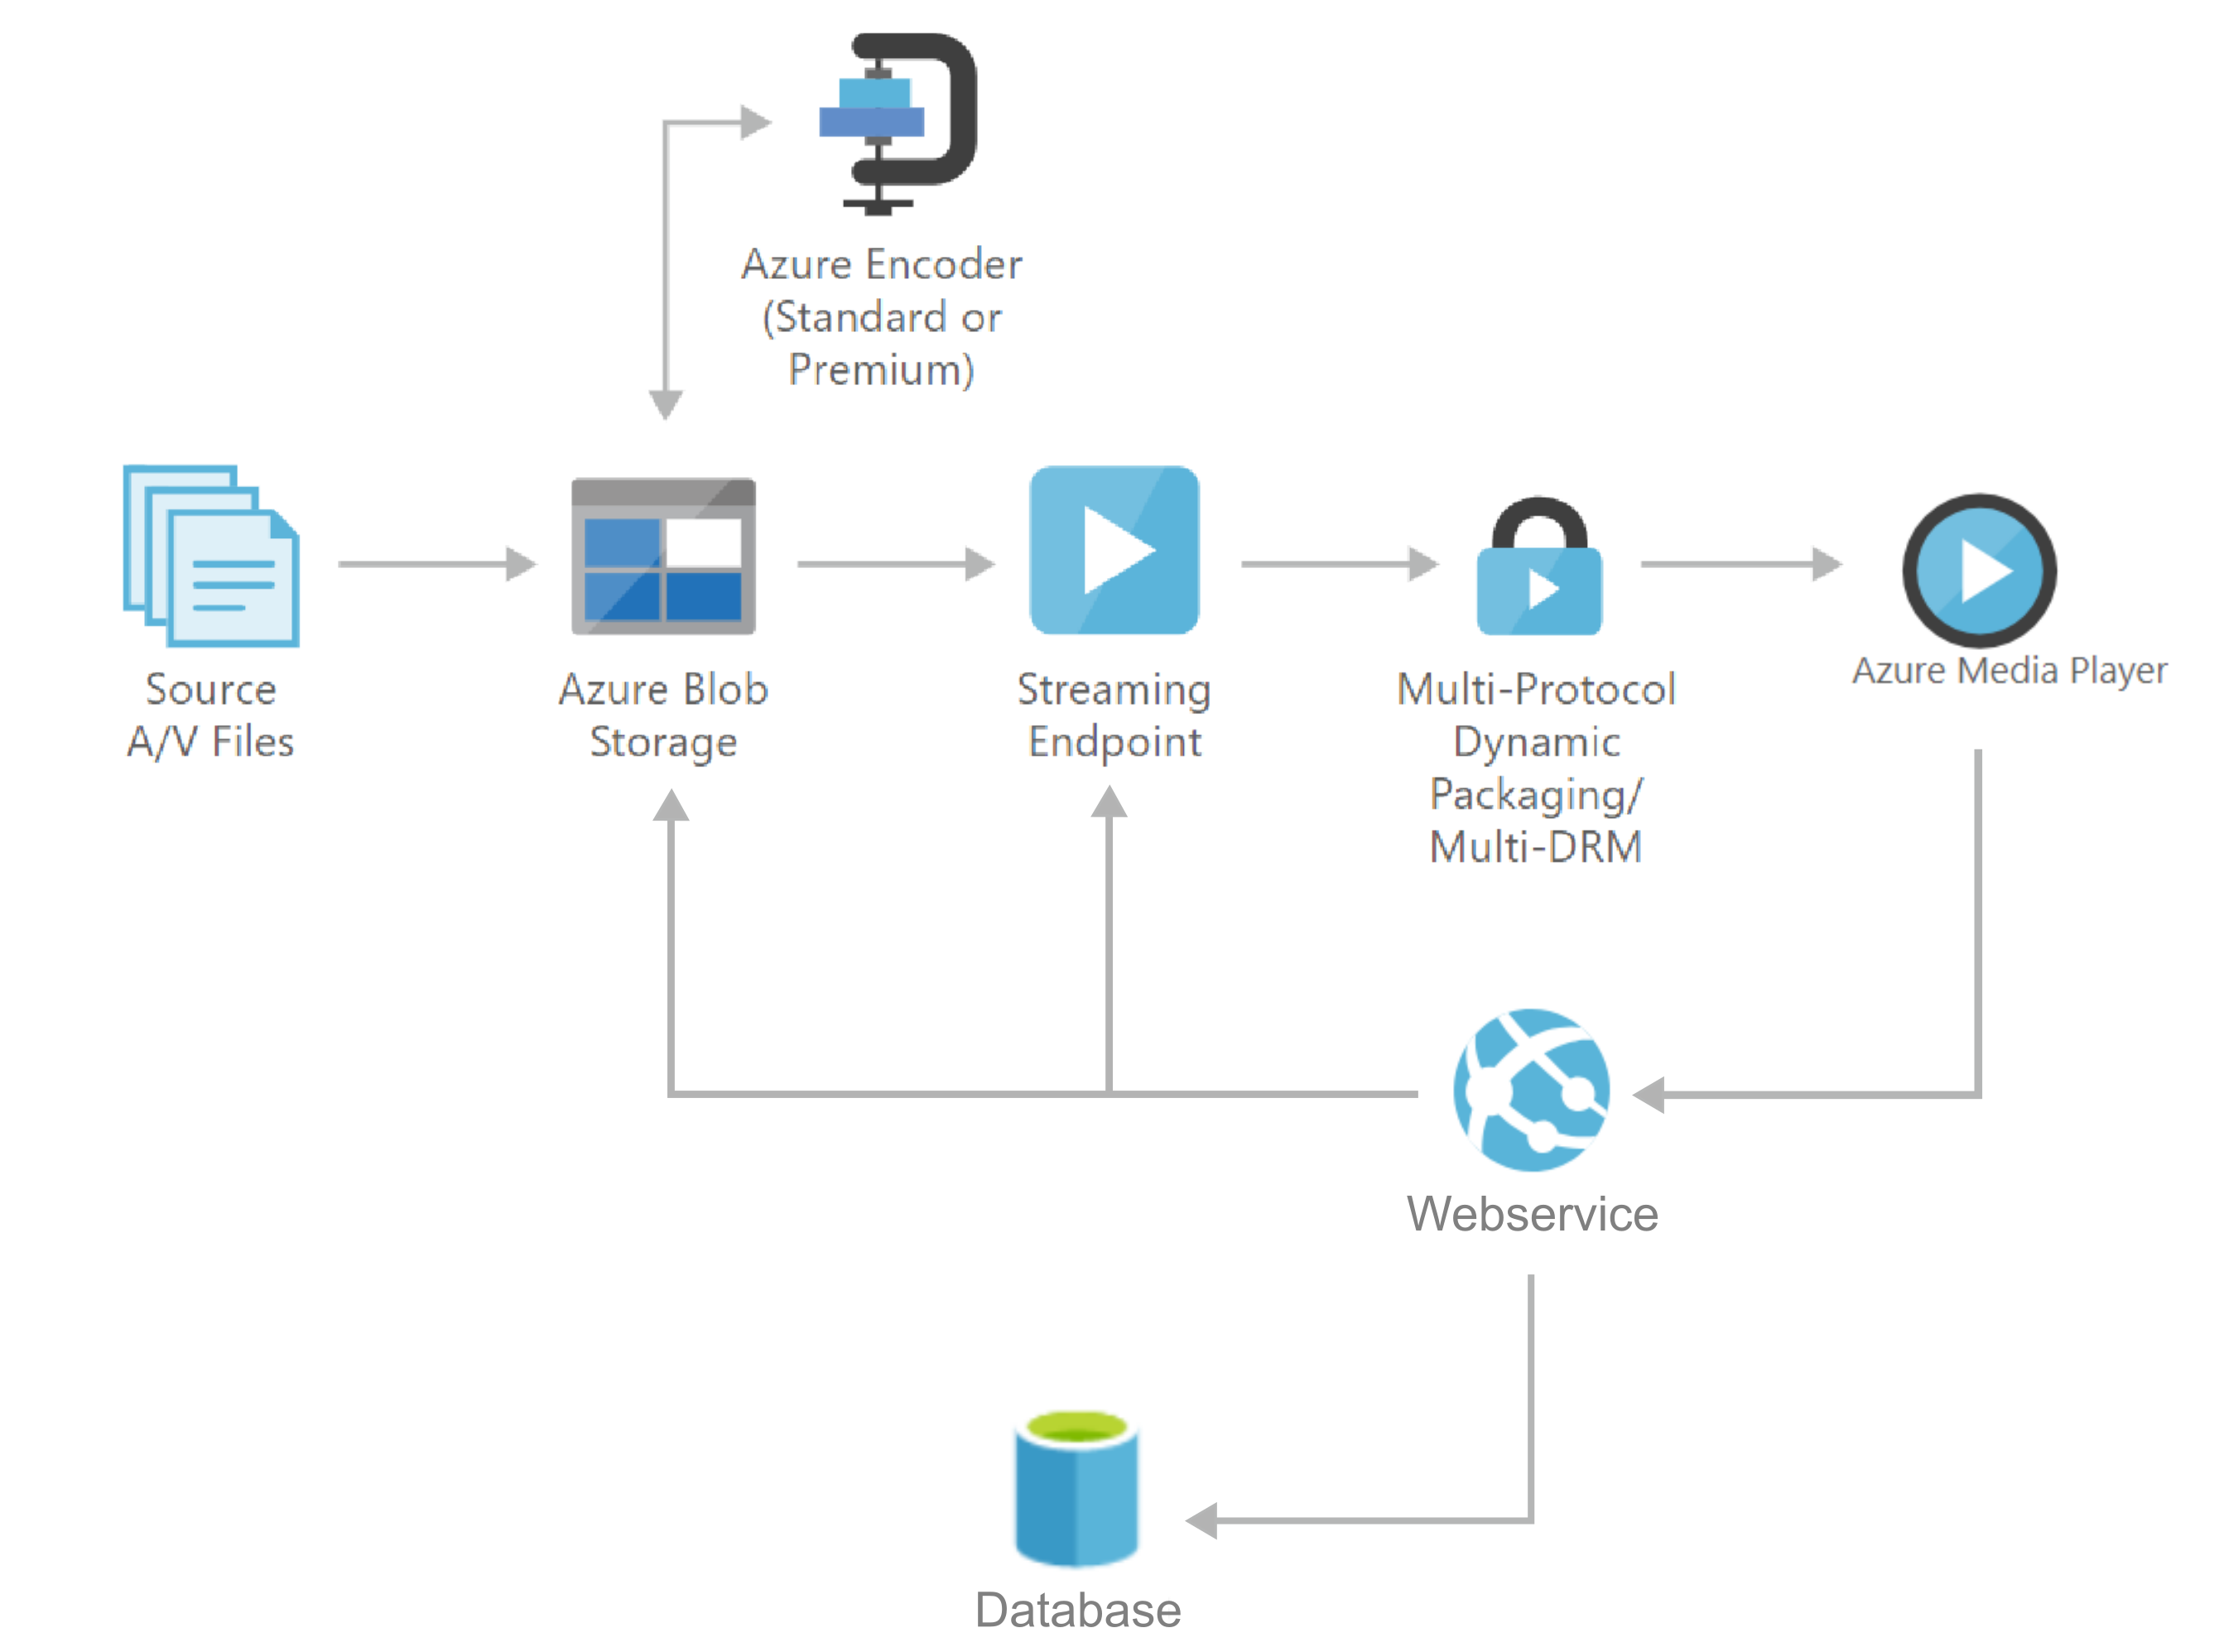
\includegraphics[height=200px]{ressources/architecture_new.png}  %[width=1\pagewidth, height=240px]
    \caption{Modified implementation of Microsofts VoD architecture}
    \label{fig:arch_new}
  \end{figure}
% ACuch benötigt laut config.js:  Azure ActiveDirectory (aad) id, secret, tenantID
% das hier?    https://docs.microsoft.com/de-de/azure/active-directory/develop/howto-create-service-principal-portal#create-an-azure-active-directory-application
% jap, steht in depl-script, auskommentiert. einmalige ausführung

Using Media Services results in a \textit{two-tier} server-architecture, in 
which the NodeJS-powered AppService has the end-user's devices as clients. The 
webserver itself is a client to the Azure Media Services Backend, requesting 
Encoding- and Streaming-Tasks by submitting \textit{Jobs}. This is also for 
security reasons, as Media Services uses a separate account-system with it's 
own credentials, generated by Microsoft. Those are confidential and must not be
exposed to end-users. CORS (Cross Origin Resource Sharing) must also be enabled for 
the Storage Account. 

The cloud components scale completely automatic as needed. The NodeJS 
AppService is configured to scale along the workload of the CPU resulting in 
creating another instance of the service. This happens once the defined 
threshold is reached. Incoming requests will automatically distributed by Azure 
using the free Load Balancer Service. 
The database and Blob Storage behave in the same way, scaling up and down when 
needed depending on the used price tier.